\section{Results and Discussion}\label{results-and-discussion}

This chapter reports the confirmatory empirical results of the
\textbf{Graph-Based Bounded Risk Propagation Model (GBBRPM)} executed
under the frozen \texttt{v2.0.0-protocol-freeze} release
(\texttt{0b986e4}) and archived in the \texttt{v2.0.0-heldout-eval}
evaluation bundle (\texttt{76ae58c}). Every metric, uncertainty
interval, and assertion in Sections~4.1--4.8 was produced strictly from
the frozen benchmark harness, scalability suite, and real-domain
instantiation scripts specified in Chapter~3 without altering core
model equations or tuning parameters after held-out evaluation began.
Historical preliminary evidence from the September~2026 N1--N5
136-scenario study and the exploratory SWMM hydraulic-mismatch study is
intentionally kept separate and preserved in
\hyperref[app:preliminary]{Appendix D} so that confirmatory held-out
outcomes and earlier exploratory diagnostics are never conflated.

\subsection{Protocol Freeze Execution, Hard Invariant Verification, and Inventory Audit}
\label{sec:v2-protocol-audit}

Before any held-out evaluation seed (\texttt{1001--1020}) was executed,
the complete computational contract---covering the core engine,
Compressed Sparse Row (CSR) kernels, synthetic DAG generators, exact
enumeration and bit-packed Monte Carlo references, matched comparators,
Two-Stage Deterministic Certified Top-$k$ Screening, and frozen public
inputs---was locked under Git tag \texttt{v2.0.0-protocol-freeze} with
a cryptographic SHA-256 manifest spanning \texttt{35/35} tracked files
(plus external SHA-256 verification of the restricted DPWH and Caltech
source archives without exporting restricted payloads into version
control). Automated pre-freeze verification confirmed \texttt{88/88}
passing tests in the core \texttt{pytest} suite, \texttt{5/5} passing
legacy analytical/behavioral verification scripts, and \texttt{76/76}
passing automated checks in the interactive research prototype
(\texttt{gbbrpm-prototype}), establishing fail-closed rejection of
cycles, self-loops, non-finite inputs, and dual $S+L/C$ specifications,
exact numerical parity between the reference DataFrame engine and the
CSR implementation (maximum discrepancy $0.0$), and exact replay
traceability (\hyperref[app:prototype-contract]{Appendix E}).

A pre-freeze development compute pilot ($54$ timed configurations on
development seed \texttt{41}, peak traced heap memory $46.49\text{ MB}$,
elapsed runtime $25.27\text{ s}$) measured bit-packed Monte Carlo
throughput of $219.95\text{ million}$ edge-trials/s at $|V|=250$ and
extrapolated $26.30\text{ min}$ single-core ($4.38\text{ min}$ on
$8$ workers) for the full $4,316$-scenario primary inventory
($88.86\text{ billion}$ edge-trials). Because the full inventory proved
feasible without scenario reduction, no pre-registered protocol scope
was pruned. Executing the entire held-out evaluation bundle
($3,060$ total evaluations across held-out uniform DAGs, held-out
heterogeneous DAGs, stochastic \texttt{Express 4.18.2}, and independent
$N=1{,}000{,}000$ precision audits) required $175.59\text{ s}$
($2.93\text{ min}$) on $8$ CPU workers under Python~3.13.14 on
Windows~11 (12 logical AMD64 cores), with all \texttt{35/35} frozen
file hashes passing pre-run verification.

% Auto-generated by scripts/generate_paper_outputs.py --target thesis; do not edit manually.
\begin{table}[htbp]
\centering
\caption{Frozen v2.0.0 experimental inventory, split discipline, and hard protocol assertions.}
\label{tab:v2-inventory-assertions}
\footnotesize
\setlength{\tabcolsep}{4.0pt}
\resizebox{\linewidth}{!}{%
\begin{tabular}{llrrccc}
\toprule
Suite & Split / Seeds & Scenarios & Reference & Bracket viol. & False certs & Empty CI nodes \\
\midrule
Matched branch controls & Dev / exact & 560 & Eq. (3-15) exact & 0 & 0 & 0 \\
Uniform DAG controls & Dev (41--45) & 720 & 100k MC ($60$ graphs) & 0 & 0 & 1 \\
Heterogeneous DAG controls & Dev (41) & 24 & 100k MC ($12$ graphs) & 0 & 0 & 0 \\
Held-out uniform DAGs & Eval (1001--1020) & 2,880 & 100k MC ($240$ graphs) & 0 & 0 & 1 \\
Held-out heterogeneous DAGs & Eval (1001--1005) & 120 & 100k MC ($60$ graphs) & 0 & 0 & 0 \\
Express 4.18.2 stochastic & Real topology & 12 & 100k MC (71N/128E) & 0 & 0 & 0 \\
\midrule
\textbf{Primary inventory total} & \textbf{Dev + Eval} & \textbf{4,316} & \textbf{88.86B edge-trials} & \textbf{0} & \textbf{0} & 2 \\
Precision audits (1M MC) & Eval (1001) & 48 & 1M MC (indep. seed) & 0 & 0 & 0 \\
Real-domain instantiations & 3 domains & 115 & Exact / 100k MC & 0 & 0 & 0 \\
\bottomrule
\end{tabular}
}
\par\vspace{3pt}\parbox{0.98\linewidth}{\raggedright\scriptsize Bracket violations check $M_j \le T_j \le R_j \le H_j$ across all nodes (tolerance $10^{-12}$). False certifications cover Stage 1 and Stage 2 across $f \in \{0.10, 0.20, 0.30\}$ against both analytic $[T_j,R_j]$ and nonempty intersected intervals. Empty Hoeffding intersections are recorded transparently without silent repair (1 non-candidate source node in dev; 1 non-candidate source node in held-out; 0 candidate nodes).}
\end{table}


Table~\ref{tab:v2-inventory-assertions} summarizes the complete frozen
v2.0.0 inventory and hard mathematical invariant assertions. Across all
$4,316$ primary benchmark scenarios ($1,304$ development controls and
$3,012$ held-out/real-topology runs), all $48$ independent $1\text{M}$-trial
precision audits, and all $115$ real-domain instantiation scenarios
($4,479$ evaluations in total), the study recorded \textbf{zero}
receiving-state bracket violations ($M_j \le T_j \le R_j \le H_j$
within $10^{-12}$ tolerance), \textbf{zero} \citet{abbe2020} lower-bound
violations, and \textbf{zero} false top-$k$ certifications across every
tested budget fraction $f \in \{0.10, 0.20, 0.30\}$ against both the
analytic $[T_j, R_j]$ bracket and nonempty Hoeffding-intersected
reference intervals.

Consistent with the preregistered non-repair policy
(Section~\ref{analysis-reproducibility}), empty intersections between
the analytic bracket $[T_j, R_j]$ and the $95\%$ union-bound Hoeffding
interval $[\hat{\pi}_j - h, \hat{\pi}_j + h]$ were logged without
silent clamping. Across all $3,012$ primary held-out evaluations,
exactly \textbf{one} node produced an empty Hoeffding intersection
(scenario \texttt{dag\_\allowbreak uniform|\allowbreak eval|\allowbreak layered|\allowbreak n=250|\allowbreak seed=1003|\allowbreak w=0.25|\allowbreak B=0.5},
occurring on a non-candidate source node with $B_j > 0$, leaving
\textbf{zero} affected candidate nodes in $C=\{B_j=0\}$), mirroring
one non-candidate source node in the $720$ development controls and
\textbf{zero} empty intersections across all $48$ independent
$1\text{M}$-trial precision audits. At a $5\%$ family-wise Hoeffding
tail rate across thousands of scenarios, two non-candidate tail
excursions in $4,316$ runs lie well below the conservative union bound
and confirm statistical honesty rather than bracket failure.

\subsection{Matched Shared-vs.-Independent Branch Dependence Controls}
\label{sec:v2-matched-branch}

To isolate shared-ancestry collapse from topology noise, the
$560$-scenario matched branch control suite evaluated paired
shared-origin and independent-origin branch families across branch
counts $m \in \{1, 2, 4, 8\}$, path lengths $\ell \in \{2, 4\}$,
effective edge weights $p \in \{0.05, 0.10, 0.20, 0.25, 0.50, 0.75, 1.00\}$,
and local source severities $b \in \{0.10, 0.25, 0.50, 0.75, 1.00\}$,
using the exact closed-form reference of Equation~(3-15) and
cross-checking $404$ tractable instances against direct state-space
enumeration with zero discrepancies.

\begin{figure}[htbp]
\centering
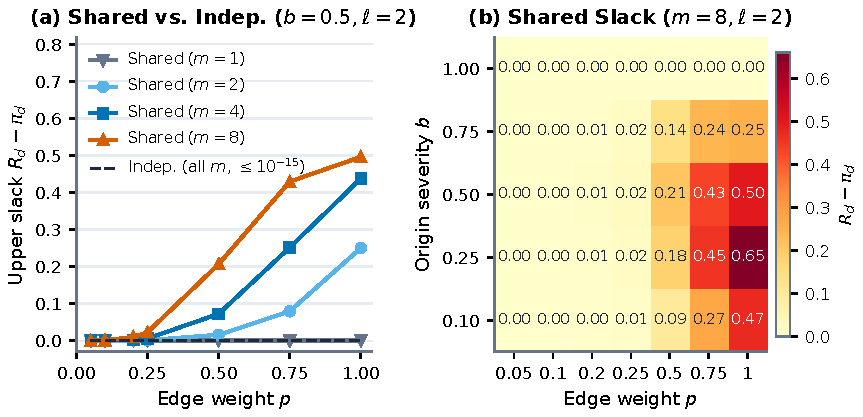
\includegraphics[width=0.96\textwidth]{figures/v2/fig_v2_matched_branch_controls.pdf}
\caption{Matched shared-origin versus independent-origin branch dependence controls ($560$ exact scenarios): exact agreement under independent origins versus bounded one-sided upper slack $R_j - \pi_j$ under uncertain shared origins ($0 < b < 1$) and exact collapse to zero at $b = 1$.}
\label{fig:v2-matched-branch}
\end{figure}

Figure~\ref{fig:v2-matched-branch} confirms every analytical prediction
of Hypothesis~$H_1$ under exact reference probabilities:
\begin{enumerate}[label=\arabic*.,leftmargin=*]
\item \textbf{Exact Equivalence Under Independent Origins.} Across all
$280$ independent-origin scenarios, GBBRPM ($R_j$) and the
target-specific in-arborescence bound ($T_j$) coincided identically with
exact $\pi_j$: maximum upper slack was $1.11 \times 10^{-16}$
(floating-point machine epsilon), mean tree width $R_j - T_j$ was $0.0$,
mean fixed-budget selection regret at $f=0.20$ was $1.17 \times 10^{-17}$,
and \textbf{zero} pairwise rank reversals occurred. By contrast, even
under independent origins, the \citet{abbe2020} DAG lower bound
exhibited mean lower slack $0.0792$ because its path-decay formulation
is more conservative than exact tree recursion.
\item \textbf{Controlled Shared-Origin Divergence at Intermediate $b$.}
Across the $280$ matched shared-origin scenarios, the receiver node's
true probability $\pi_j$ fell strictly below $R_j$ whenever $0 < b < 1$
and $m \ge 2$, producing mean upper slack $R_j - \pi_j = 0.0447$ and a
peak divergence of $0.6499$ ($0.649887$, occurring under high fan-out
$m=8$, high transmission, and uncertain source $b$). Mean lower slack
was $0.0500$ for $T_j$ and $0.0345$ for the \citet{abbe2020} bound,
with zero Abbe lower-bound violations. Unequal shared-origin slack
produced interval-resolved pairwise rank reversals in $23/280$ shared
scenarios ($8.21\%$), while mean fixed-budget selection regret for $R_j$
at $f=0.20$ remained small at $0.00157$.
\item \textbf{Exact Collapse at Deterministic Sources ($b = 1$) and
Monotone $W_j$ Alignment.} Whenever the shared origin was deterministic
($b = 1$), the incoming branches became conditionally independent
given the active source, causing $R_j - \pi_j$ to collapse identically
to $0.0$. Furthermore, within these controlled branch topologies where
reconvergence is the sole source of multi-branch width, the nodewise
Spearman correlation between the zero-cost scalar width
$W_j = R_j - M_j$ and true upper slack $R_j - \pi_j$ equaled
$1.0000$ across all matched instances.
\end{enumerate}

\subsection{Held-Out Uniform-DAG Bracket Tightness and Comparator Ranking}
\label{sec:v2-tightness-ranking}

The primary confirmatory benchmark evaluated $2,880$ held-out uniform-weight
DAG scenarios spanning $240$ independent graph replicates ($20$ held-out
seeds \texttt{1001--1020} $\times$ $3$ topology families: Forward,
Layered, and Preferential Attachment $\times$ $4$ graph sizes
$|V| \in \{20, 50, 100, 250\}$), each tested across $6$ uniform edge
weights $w \in \{0.05, 0.10, 0.20, 0.25, 0.50, 0.75\}$ and $2$ source
severities $B \in \{0.50, 1.00\}$ against $N=100{,}000$-trial bit-packed
Monte Carlo references. To avoid pseudo-replication across correlated
parameterizations of the same graph, all headline descriptive
statistics were computed at the independent graph-replicate level
($n=240$ overall; $n=20$ per family $\times$ size stratum) after
averaging the $12$ $(w, B)$ conditions per topology.

% Auto-generated by scripts/generate_paper_outputs.py --target thesis; do not edit manually.
\begin{table}[htbp]
\centering
\caption{Held-out (2,880 scenarios; 240 graph replicates) receiving-state bracket widths and slacks by family and size.}
\label{tab:v2-bracket-tightness}
\footnotesize
\setlength{\tabcolsep}{4.0pt}
\resizebox{\linewidth}{!}{%
\begin{tabular}{lrrrrrr}
\toprule
Family & $|V|$ & $W_j$ (Mean $\pm$ SD) & $W_j$ (Med. [IQR]) & $R_j - T_j$ (Mean $\pm$ SD) & $R_j - \pi_j$ (Mean $\pm$ SD) & $\pi_j - T_j$ (Mean $\pm$ SD) \\
\midrule
Forward & 20 & 0.0509 $\pm$ 0.0170 & 0.0482 [0.0160] & 0.0308 $\pm$ 0.0102 & 0.0084 $\pm$ 0.0028 & 0.0223 $\pm$ 0.0080 \\
Forward & 50 & 0.0540 $\pm$ 0.0116 & 0.0522 [0.0113] & 0.0142 $\pm$ 0.0054 & 0.0029 $\pm$ 0.0013 & 0.0112 $\pm$ 0.0042 \\
Forward & 100 & 0.0527 $\pm$ 0.0099 & 0.0553 [0.0121] & 0.0073 $\pm$ 0.0019 & 0.0014 $\pm$ 0.0004 & 0.0060 $\pm$ 0.0015 \\
Forward & 250 & 0.0572 $\pm$ 0.0090 & 0.0559 [0.0089] & 0.0038 $\pm$ 0.0007 & 0.0006 $\pm$ 0.0001 & 0.0031 $\pm$ 0.0006 \\
\midrule
Layered & 20 & 0.1092 $\pm$ 0.0202 & 0.1112 [0.0309] & 0.0711 $\pm$ 0.0170 & 0.0111 $\pm$ 0.0020 & 0.0599 $\pm$ 0.0154 \\
Layered & 50 & 0.1494 $\pm$ 0.0140 & 0.1487 [0.0197] & 0.0810 $\pm$ 0.0112 & 0.0071 $\pm$ 0.0015 & 0.0740 $\pm$ 0.0112 \\
Layered & 100 & 0.1532 $\pm$ 0.0136 & 0.1554 [0.0147] & 0.0736 $\pm$ 0.0105 & 0.0045 $\pm$ 0.0014 & 0.0692 $\pm$ 0.0103 \\
Layered & 250 & 0.1387 $\pm$ 0.0088 & 0.1366 [0.0108] & 0.0759 $\pm$ 0.0073 & 0.0033 $\pm$ 0.0007 & 0.0726 $\pm$ 0.0071 \\
\midrule
Pref. Att. & 20 & 0.1491 $\pm$ 0.0085 & 0.1465 [0.0115] & 0.0863 $\pm$ 0.0077 & 0.0194 $\pm$ 0.0019 & 0.0669 $\pm$ 0.0063 \\
Pref. Att. & 50 & 0.1425 $\pm$ 0.0072 & 0.1425 [0.0082] & 0.0477 $\pm$ 0.0073 & 0.0067 $\pm$ 0.0012 & 0.0411 $\pm$ 0.0071 \\
Pref. Att. & 100 & 0.1444 $\pm$ 0.0041 & 0.1448 [0.0049] & 0.0286 $\pm$ 0.0035 & 0.0044 $\pm$ 0.0008 & 0.0242 $\pm$ 0.0029 \\
Pref. Att. & 250 & 0.1484 $\pm$ 0.0029 & 0.1493 [0.0034] & 0.0198 $\pm$ 0.0024 & 0.0022 $\pm$ 0.0003 & 0.0176 $\pm$ 0.0023 \\
\midrule
\textbf{Overall} & \textbf{240} & \textbf{0.1125 $\pm$ 0.0445} & \textbf{0.1374 [0.0868]} & \textbf{0.0450 $\pm$ 0.0310} & \textbf{0.0060 $\pm$ 0.0052} & \textbf{0.0390 $\pm$ 0.0278} \\
\bottomrule
\end{tabular}
}
\par\vspace{3pt}\parbox{0.98\linewidth}{\raggedright\scriptsize Statistics are computed over independent graph replicates ($n=20$ per family $\times$ size stratum; $n=240$ overall) after averaging across the 12 $(w, B)$ conditions on each topology.}
\end{table}


\begin{figure}[htbp]
\centering
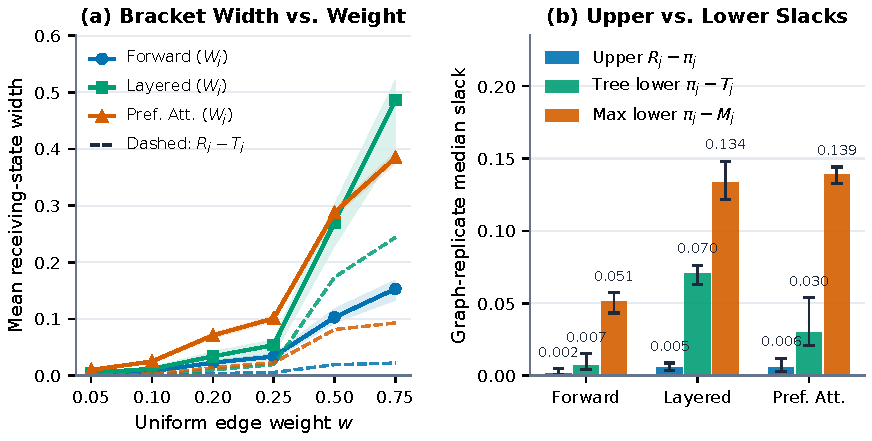
\includegraphics[width=0.96\textwidth]{figures/v2/fig_v2_bracket_tightness.pdf}
\caption{Held-out uniform-DAG receiving-state bracket tightness ($2,880$ scenarios; $240$ graph replicates): decomposition of scalar width $W_j = R_j - M_j$ and tree width $R_j - T_j$ into upper slack $R_j - \pi_j$ and lower slack $\pi_j - T_j$ across topology families, graph sizes, and weight regimes.}
\label{fig:v2-bracket-tightness}
\end{figure}

Table~\ref{tab:v2-bracket-tightness} and
Figure~\ref{fig:v2-bracket-tightness} reveal a striking asymmetry inside
the analytic receiving-state bracket $M_j \le T_j \le \pi_j \le R_j$:
across all $240$ held-out graph replicates, the mean scalar bracket
width was $W_j = R_j - M_j = 0.1125 \pm 0.0445$ (median $0.1374$,
IQR $0.0868$), which Stage~2 tree refinement compressed by $60.0\%$ to
mean tree width $R_j - T_j = 0.0450 \pm 0.0310$. Crucially,
\textbf{$86.7\%$ of the tree width lay below $\pi_j$} (mean lower slack
$\pi_j - T_j = 0.0390 \pm 0.0278$; mean $\pi_j - M_j = 0.1065$), while
GBBRPM's actual mean one-sided upper slack was only
$R_j - \pi_j = 0.0060 \pm 0.0052$ (mean MAE $0.00636$, versus $0.0392$
for $T_j$ and $0.0466$ for \citealp{abbe2020}).

Stratification by topology, edge weight, and source uncertainty
confirms the dependence mechanisms predicted by $H_1$:
\begin{itemize}[leftmargin=*]
\item \textbf{Topology Family and Size:} Forward DAGs exhibited the
tightest brackets ($W=0.0537$, $R-T=0.0140$, $R-\pi=0.00334$), whereas
Layered DAGs ($W=0.1376$, $R-T=0.0754$, $R-\pi=0.00650$) and
Preferential Attachment DAGs ($W=0.1461$, $R-T=0.0456$,
$R-\pi=0.00815$) incurred wider brackets due to denser shared-ancestry
reconvergence. Upper slack $R_j - \pi_j$ decreased monotonically with
graph size $|V|$ across all three families (e.g., from $0.0194$ at
$|V|=20$ to $0.0022$ at $|V|=250$ in Preferential Attachment) as
multi-hop attenuation diluted distant shared origins across fixed-degree
sparse DAGs.
\item \textbf{Edge Weight ($w$) and Source Uncertainty ($B$):} Mean
upper slack remained near zero under strong attenuation ($R-\pi < 0.00002$
at $w=0.05$ and $w=0.10$; $0.00039$ at $w=0.20$; $0.00091$ at $w=0.25$),
rising substantially only in high-transmission regimes ($0.01243$ at
$w=0.50$ and $0.02221$ at $w=0.75$, with worst-case single-node slack
$0.4203$ and peak $W_{\max}=0.9870$). Consistent with the conditional
independence mechanism at certain sources, mean upper slack under
uncertain sources ($B=0.50$, $R-\pi = 0.01080$) was $9.1\times$ larger
than under deterministic sources ($B=1.00$, $R-\pi = 0.00119$).
\end{itemize}

% Auto-generated by scripts/generate_paper_outputs.py --target thesis; do not edit manually.
\begin{table}[htbp]
\centering
\caption{Held-out (2,880 scenarios; 240 replicates) fixed-budget regret, capture, and rank correlation across comparators.}
\label{tab:v2-comparator-ranking}
\footnotesize
\setlength{\tabcolsep}{4.0pt}
\resizebox{\linewidth}{!}{%
\begin{tabular}{lrrrrrr}
\toprule
Comparator & Regret $f=0.10$ & Regret $f=0.20$ & Regret $f=0.30$ & Capture $f=0.20$ & Spearman $\rho$ & $\Delta\mathrm{Regret}_{0.20}$ ($R$ wins) \\
\midrule
GBBRPM ($R_j$) & 0.0055 $\pm$ 0.0062 & 0.0074 $\pm$ 0.0075 & 0.0092 $\pm$ 0.0084 & 50.59\% & 0.9833 $\pm$ 0.0143 & -- \\
Tree lower ($T_j$) & 0.0670 $\pm$ 0.0808 & 0.1483 $\pm$ 0.2402 & 0.2535 $\pm$ 0.4409 & 49.97\% & 0.8992 $\pm$ 0.0738 & -0.1409 (97.5\%) \\
Abbe lower & 0.1740 $\pm$ 0.2003 & 0.2968 $\pm$ 0.3719 & 0.4034 $\pm$ 0.5177 & 49.80\% & 0.9149 $\pm$ 0.0540 & -0.2894 (98.3\%) \\
Clipped sum ($H_j$) & 0.2288 $\pm$ 0.2222 & 0.2889 $\pm$ 0.2729 & 0.2969 $\pm$ 0.3022 & 49.99\% & 0.9554 $\pm$ 0.0263 & -0.2814 (100.0\%) \\
Ancestry diag. & 0.3204 $\pm$ 0.2889 & 0.5590 $\pm$ 0.5155 & 0.6350 $\pm$ 0.6165 & 47.31\% & 0.8586 $\pm$ 0.0739 & -0.5516 (99.6\%) \\
Local-upstream & 0.4041 $\pm$ 0.5114 & 0.9185 $\pm$ 1.2449 & 1.2314 $\pm$ 1.6721 & 45.65\% & 0.6810 $\pm$ 0.1681 & -0.9110 (98.8\%) \\
Recursive max ($M_j$) & 0.6700 $\pm$ 0.6269 & 0.9332 $\pm$ 0.8222 & 0.9417 $\pm$ 0.8022 & 45.30\% & 0.8198 $\pm$ 0.0801 & -0.9257 (99.6\%) \\
\bottomrule
\end{tabular}
}
\par\vspace{3pt}\parbox{0.98\linewidth}{\raggedright\scriptsize Graph-replicate means $\pm$ SD ($n=240$). Negative $\Delta\mathrm{Regret}_{0.20} = \mathrm{Regret}(R) - \mathrm{Regret}(\text{comp})$ indicates lower regret for GBBRPM ($R_j$); parentheses give percentage of replicates where $R_j$ strictly achieves lower regret. Interval-resolved pairwise reversals for $R_j$: pooled rate 0.198\% (37,489 / 18,943,293 resolved strict pairs; 696/2,880 scenarios).}
\end{table}


\begin{figure}[htbp]
\centering
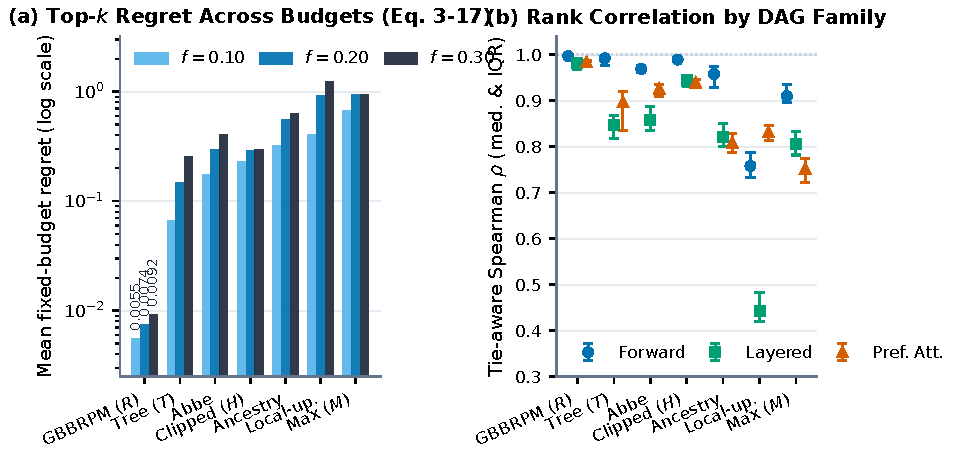
\includegraphics[width=0.96\textwidth]{figures/v2/fig_v2_fixed_budget_ranking.pdf}
\caption{Fixed-budget top-$k$ selection regret ($\operatorname{Regret}_k$), captured activation mass, and rank correlation across GBBRPM ($R_j$) and matched comparators on $2,880$ held-out uniform-DAG scenarios ($240$ graph replicates).}
\label{fig:v2-fixed-budget-ranking}
\end{figure}

Table~\ref{tab:v2-comparator-ranking} and
Figure~\ref{fig:v2-fixed-budget-ranking} report fixed-budget candidate
selection ($C = \{B_j = 0\}$, evaluated across $100$ shared
outcome-independent tie permutations using seed~\texttt{140}) and
whole-graph rank correlation against $\pi_j$. Across all three budget
fractions $f \in \{0.10, 0.20, 0.30\}$, GBBRPM ($R_j$) achieved the
lowest fixed-budget regret and highest captured activation mass among
all seven deterministic methods. At the primary $f=0.20$ budget,
GBBRPM attained mean regret $0.00742 \pm 0.0075$ (capture $50.59\%$)
and mean Spearman rank correlation $\rho = 0.9833 \pm 0.0143$,
substantially outperforming the target-specific tree lower bound $T_j$
(regret $0.1483$, $20.0\times$ higher; $\rho = 0.8992$), clipped
additive aggregation $H_j$ (regret $0.2889$, $38.9\times$ higher;
$\rho = 0.9554$), the \citet{abbe2020} DAG lower bound (regret
$0.2968$, $40.0\times$ higher; $\rho = 0.9149$), the ancestry-aware
diagnostic (regret $0.5590$, $75.3\times$ higher; $\rho = 0.8586$),
the local-upstream recursion ablation (regret $0.9185$, $123.8\times$
higher; $\rho = 0.6810$), and recursive maximum $M_j$ (regret $0.9332$,
$125.8\times$ higher; $\rho = 0.8198$). In paired graph-replicate
comparisons at $f=0.20$, $R_j$ strictly achieved lower regret than
every comparator on $97.5\%$ to $100.0\%$ of the $240$ topologies
($97.5\%$ vs.\ $T_j$, $98.3\%$ vs.\ Abbe, $98.8\%$ vs.\ local-upstream,
$99.6\%$ vs.\ ancestry and $M_j$, and $100.0\%$ vs.\ $H_j$).

Two mechanism findings explain this separation:
\begin{enumerate}[label=\arabic*.,leftmargin=*]
\item \textbf{Saturation Resistance vs.\ Clipped Additive Aggregation ($H_j$).}
Because clipped-sum aggregation ($H_j$) adds incoming contributions
linearly until hitting the hard ceiling $1.0$, $H_j$ saturated at or
above $0.95$ on $16.29\%$ of candidate nodes overall ($33.97\%$ at
$w=0.50$ and $63.61\%$ at $w=0.75$) and clipped identically at $1.0$ on
$15.84\%$ of candidates, collapsing distinct candidate tiers into
massive top-rank ties (mean $41.18$ distinct score groups vs.\ $57.35$
for $R_j$ and $74.37$ for $\pi_j$). GBBRPM's asymptotic complement
product limited $\ge 0.95$ saturation to $1.49\%$ ($0.06\%$ at $w=0.50$;
$8.89\%$ at $w=0.75$) with $0.0\%$ numerical clipping at $1.0$,
preserving ranking discrimination under heavy multi-source load.
\item \textbf{Honest Accounting of Unfavorable Reversal Regimes and
Ancestry-Diagnostic Tradeoffs.} Although GBBRPM dominated aggregate
ranking accuracy, shared-ancestry collapse still generated measurable
\emph{interval-resolved pairwise rank reversals} ($R_a > R_b$ while the
entire Hoeffding interval of $\pi_a$ lay strictly below that of $\pi_b$)
in $696/2,880$ held-out scenarios ($24.17\%$). Across all
$18,943,293$ Hoeffding-resolved strict model pairs, $37,489$ pairs
reversed, yielding a pooled reversal rate of $0.198\%$ ($0.001979$;
replicate mean $0.523\%$), while $13.30\%$ of all valid candidate pairs
($2,906,873 / 21,850,560$) remained statistically unresolved within the
$N=100{,}000$ Hoeffding margin. Reversals were heavily concentrated in
high-weight, uncertain-source regimes: $694$ of the $696$ reversal
scenarios occurred at $w \in \{0.50, 0.75\}$ ($359$ at $w=0.50$, $335$
at $w=0.75$, only $2$ at $w=0.25$, and $0$ for $w \le 0.20$), and
$466$ occurred at $B=0.50$ (pooled rate $0.313\%$) versus $230$ at
$B=1.00$ ($0.082\%$), peaking in Layered ($285$ scenarios, $0.311\%$)
and Preferential Attachment ($185$ scenarios, $0.225\%$) over Forward
DAGs ($226$ scenarios, $0.063\%$). Notably, the connected-component
ancestry diagnostic did \emph{not} outperform scalar $R_j$: by pruning
secondary paths within shared-origin components, it discarded genuine
multi-path cumulative activation and raised $f=0.20$ regret to $0.5590$.
\end{enumerate}

\subsection{Two-Stage Deterministic Certified Top-\texorpdfstring{$k$}{k} Screening and \texorpdfstring{$W_j$}{Wj} Self-Diagnosis}
\label{sec:v2-certified-screening}

Rather than relying on scalar point rankings alone when upper slack may
cause reversals, Two-Stage Deterministic Certified Top-$k$ Screening
exploits the proven bracket $M_j \le T_j \le \pi_j \le R_j$ to partition
candidates into provably certified top-$k$ inclusions ($I_k$), provably
certified exclusions ($O_k$), and an explicit uncertified boundary band
($U_k$) without executing a single Monte Carlo trial. Stage~1 applies
the $O(|V|+|E|)$ scalar bracket $[M_j, R_j]$; Stage~2 computes the
tighter target-specific in-arborescence bound $T_j$ \emph{exclusively}
for nodes surviving inside the Stage~1 boundary band $U_k^{(1)}$.

% Auto-generated by scripts/generate_paper_outputs.py --target thesis; do not edit manually.
\begin{table}[htbp]
\centering
\caption{Two-Stage Deterministic Certified Top-$k$ Screening resolution, full certification, and wall-clock speedups (held-out 2,880).}
\label{tab:v2-certified-screening}
\footnotesize
\setlength{\tabcolsep}{4.0pt}
\resizebox{\linewidth}{!}{%
\begin{tabular}{lrrrrrrr}
\toprule
Family & $f$ & $\mathrm{Res}_{S1}$ & $\mathrm{Res}_{S2}$ & $\Delta_{\mathrm{band}}$ & Full Cert. S2 & Speedup vs. $T_j$ & Speedup vs. MC \\
\midrule
Forward & 0.10 & 59.5\% $\pm$ 6.5\% & 89.6\% $\pm$ 9.7\% & +30.1 pp & 12.7\% & 2.25$\times$ [0.63] & 55.7$\times$ [40.1] \\
Forward & 0.20 & 59.9\% $\pm$ 7.8\% & 87.2\% $\pm$ 11.3\% & +27.3 pp & 15.1\% & 2.28$\times$ [0.71] & 56.4$\times$ [40.1] \\
Forward & 0.30 & 60.4\% $\pm$ 9.3\% & 85.7\% $\pm$ 9.6\% & +25.4 pp & 12.9\% & 2.26$\times$ [0.76] & 54.8$\times$ [39.0] \\
\midrule
Layered & 0.10 & 66.9\% $\pm$ 5.3\% & 85.3\% $\pm$ 6.6\% & +18.4 pp & 23.5\% & 8.26$\times$ [8.19] & 132.2$\times$ [76.3] \\
Layered & 0.20 & 58.2\% $\pm$ 6.4\% & 76.9\% $\pm$ 6.7\% & +18.7 pp & 13.8\% & 4.77$\times$ [4.31] & 81.1$\times$ [41.5] \\
Layered & 0.30 & 48.3\% $\pm$ 5.6\% & 68.8\% $\pm$ 7.3\% & +20.5 pp & 6.4\% & 2.63$\times$ [1.34] & 46.1$\times$ [40.0] \\
\midrule
Pref. Att. & 0.10 & 24.3\% $\pm$ 5.4\% & 71.6\% $\pm$ 4.5\% & +47.3 pp & 0.0\% & 1.47$\times$ [0.28] & 31.3$\times$ [30.3] \\
Pref. Att. & 0.20 & 24.3\% $\pm$ 5.4\% & 72.7\% $\pm$ 10.3\% & +48.4 pp & 19.9\% & 1.46$\times$ [0.29] & 31.7$\times$ [30.5] \\
Pref. Att. & 0.30 & 24.5\% $\pm$ 6.6\% & 61.4\% $\pm$ 11.7\% & +36.9 pp & 3.4\% & 1.48$\times$ [0.29] & 31.7$\times$ [30.4] \\
\midrule
\textbf{Overall} & \textbf{0.10} & \textbf{50.2\% $\pm$ 19.5\%} & \textbf{82.1\% $\pm$ 10.5\%} & \textbf{+31.9 pp} & \textbf{12.1\%} & \textbf{2.25$\times$ [3.56]} & \textbf{64.6$\times$ [75.1]} \\
\textbf{Overall} & \textbf{0.20} & \textbf{47.5\% $\pm$ 17.7\%} & \textbf{78.9\% $\pm$ 11.4\%} & \textbf{+31.5 pp} & \textbf{16.2\%} & \textbf{2.24$\times$ [1.93]} & \textbf{56.2$\times$ [49.8]} \\
\textbf{Overall} & \textbf{0.30} & \textbf{44.4\% $\pm$ 16.6\%} & \textbf{72.0\% $\pm$ 14.0\%} & \textbf{+27.6 pp} & \textbf{7.6\%} & \textbf{1.96$\times$ [1.09]} & \textbf{44.8$\times$ [42.8]} \\
\bottomrule
\end{tabular}
}
\par\vspace{3pt}\parbox{0.98\linewidth}{\raggedright\scriptsize Resolution rates are graph-replicate means $\pm$ SD; speedups are replicate medians [IQR]. Across all 2,880 held-out scenarios and all three budgets ($8,640$ screening evaluations), false certifications equal 0 against both analytic $[T_j,R_j]$ and intersected Hoeffding intervals.}
\end{table}


\begin{figure}[htbp]
\centering
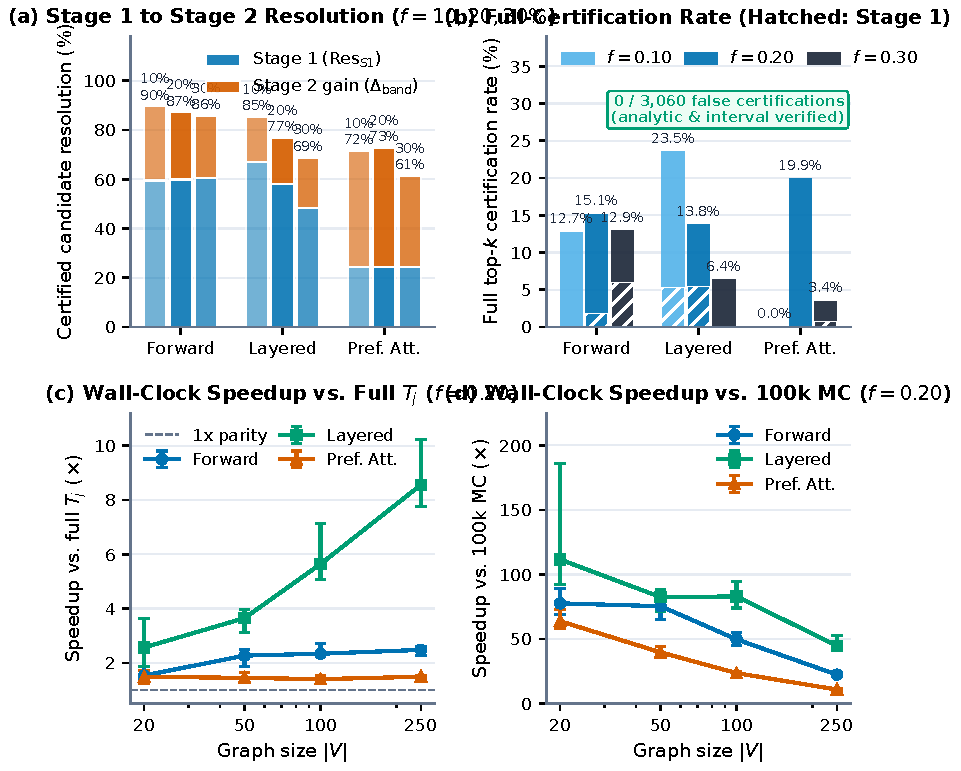
\includegraphics[width=0.96\textwidth]{figures/v2/fig_v2_certified_screening.pdf}
\caption{Two-Stage Deterministic Certified Top-$k$ Screening performance on $2,880$ held-out scenarios: Stage~1 versus Stage~2 deterministic resolution fractions, full-certification rates, and wall-clock speedups relative to full-graph $T_j$ and $N=100{,}000$ Monte Carlo.}
\label{fig:v2-certified-screening}
\end{figure}

Table~\ref{tab:v2-certified-screening} and
Figure~\ref{fig:v2-certified-screening} demonstrate the operational
effectiveness of two-stage screening across all $8,640$ held-out
screening evaluations ($2,880$ scenarios $\times$ $3$ budgets):
\begin{itemize}[leftmargin=*]
\item \textbf{Zero False Certifications and Large Boundary-Band
Contraction.} False certifications equaled \textbf{zero} across all
$8,640$ evaluations. At the primary $f=0.20$ budget, Stage~1 scalar
filtering deterministically resolved $\mathrm{Res}_{S1} = 47.5\% \pm 17.7\%$
($0.4745$) of candidate nodes in $O(|V|+|E|)$ time. Targeted Stage~2
tree refinement lifted deterministic resolution to
$\mathrm{Res}_{S2} = 78.9\% \pm 11.4\%$ ($0.7891$)---a $+31.5\text{ pp}$
($+0.3146$) boundary-band contraction---and expanded full top-$k$
certification ($|U_k^{(2)}| = 0$, requiring zero downstream MC work)
nearly sevenfold from $2.43\%$ in Stage~1 to $16.25\%$ ($16.2\%$) in
Stage~2. Similar gains held at $f=0.10$ ($\mathrm{Res}_{S1}=50.2\% \to
\mathrm{Res}_{S2}=82.1\%$, $+31.9\text{ pp}$, $12.1\%$ full cert.) and
$f=0.30$ ($\mathrm{Res}_{S1}=44.4\% \to \mathrm{Res}_{S2}=72.0\%$,
$+27.6\text{ pp}$, $7.6\%$ full cert.).
\item \textbf{Topology-Dependent Gains and Wall-Clock Speedups.}
Stage~2 refinement delivered its largest resolution lift in Preferential
Attachment DAGs ($24.3\% \to 72.7\%$ at $f=0.20$, $+48.4\text{ pp}$,
$19.9\%$ full cert.), where Stage~1 scalar $M_j$ is loose on hub-fed
paths but targeted $T_j$ tightens dramatically. Forward DAGs reached
$87.2\%$ Stage~2 resolution ($89.6\%$ at $f=0.10$), while Layered DAGs
reached $76.9\%$ ($85.3\%$ at $f=0.10$, $23.5\%$ full cert.). Across
all $2,880$ held-out scenarios at $f=0.20$, restricting $T_j$
construction to $U_k^{(1)}$ achieved an aggregate wall-clock speedup of
\textbf{$2.00\times$} ($1.997\times$; scenario median $1.79\times$,
graph-replicate median $2.24\times$, up to $8.26\times$ on Layered
$f=0.10$) over full-graph $T_j$ evaluation and \textbf{$18.6\times$}
($18.65\times$; scenario median $43.3\times$, replicate median
$56.2\times$) over bit-packed $100\text{k}$ Monte Carlo.
\item \textbf{High-Weight Limit.} Under heavy transmission ($w=0.75$),
Stage~2 resolution fell to $53.75\%$ (versus $90.11\%$ at $w=0.05$ and
$88.13\%$ at $w=0.20$), leaving nearly half of candidates inside
$U_k^{(2)}$ for optional targeted Monte Carlo escalation.
\end{itemize}

\begin{figure}[htbp]
\centering
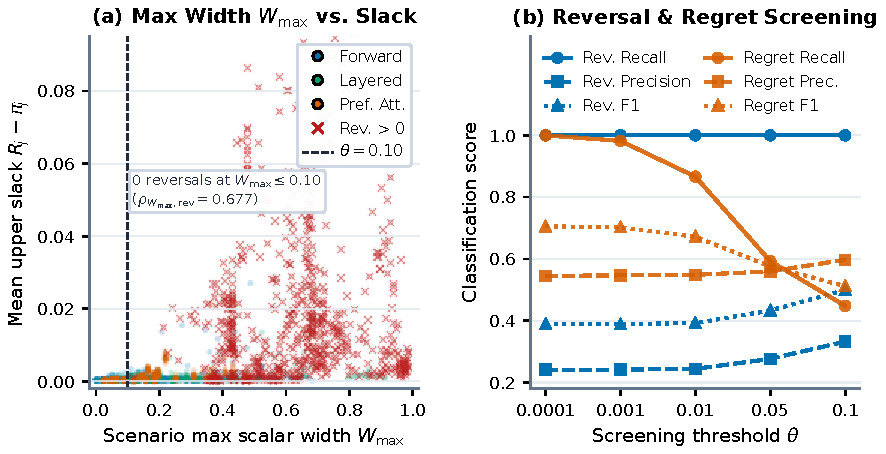
\includegraphics[width=0.96\textwidth]{figures/v2/fig_v2_w_self_diagnosis.pdf}
\caption{Evaluation of the zero-cost scalar bracket width $W_j = R_j - M_j$ as a self-diagnosing reliability indicator across $2,880$ held-out scenarios: strong scenario-level reversal screening ($\rho = 0.6769$) contrasted with modest within-graph nodewise slack correlation ($\rho = 0.2286$).}
\label{fig:v2-w-self-diagnosis}
\end{figure}

Figure~\ref{fig:v2-w-self-diagnosis} presents a nuanced empirical
verdict on Hypothesis~$H_4$ regarding the zero-cost scalar width
$W_j = R_j - M_j$. At the \textbf{scenario screening level}, the
maximum scalar width $W_{\max}$ proved to be a strong, conservative
alarm for interval-resolved rank reversals: Spearman rank correlation
between $W_{\max}$ and continuous scenario reversal rate was
\textbf{$\rho = 0.6769$} ($0.67686$) across all $2,880$ held-out
scenarios. Thresholding at $W_{\max} \ge 0.10$ achieved \textbf{$100.0\%$
recall} ($696/696$ reversal-bearing scenarios detected, \textbf{zero}
false negatives) while safely clearing $27.4\%$ of scenarios
($788/2,880$ flagged negative, precision $33.3\%$, $F_1 = 0.499$).

By contrast, at the \textbf{within-graph nodewise level} and for
continuous fixed-budget regret, $W_j$ exhibited only modest rank
association: graph-replicate mean nodewise Spearman correlation between
$W_j$ and actual upper slack $R_j - \pi_j$ was \textbf{$\rho = 0.2286$}
(SD $0.1507$, median $0.2602$, IQR $0.2430$; scenario-level median
$0.1702$), and scenario-level Spearman correlation with continuous
$f=0.20$ regret was $\rho = 0.2815$ using $W_{\mathrm{mean}}$
($\rho = 0.2839$ using boundary-band $W$). The mathematical explanation
is directly visible in Table~\ref{tab:v2-bracket-tightness}: $W_j =
(R_j - \pi_j) + (\pi_j - M_j)$ sums both shared-ancestry overestimation
($R_j - \pi_j$, mean $0.0060$) and legitimate \emph{independent}
multi-branch convergence ($\pi_j - M_j$, mean $0.1065$). Because
$\pi_j - M_j$ dominates $W_j$ by an order of magnitude on multi-source
DAGs, a node fed by several independent parents acquires a large $W_j$
even when its true upper slack $R_j - \pi_j$ is negligible. Consequently,
$W_j$ functions reliably as a \emph{necessary high-recall regime alarm}
(small $W_{\max}$ certifies low reversal risk), whereas ranking exact
nodewise slack or certifying individual top-$k$ boundaries requires
Stage~2 $T_j$ refinement.

\subsection{Weight-Heterogeneity Sensitivity and Million-Trial Precision Audits}
\label{sec:v2-hetero-audits}

Two targeted confirmatory suites tested whether the uniform-weight
results were sensitive to edge-weight dispersion or finite-sample
$N=100{,}000$ Monte Carlo noise: (a)~the $120$-scenario held-out
heterogeneous-weight suite ($60$ graph replicates across seeds
\texttt{1001--1005}, assigning deterministic SHA-256 edge weights
$w \in \{0.10, 0.20, 0.30\}$ with exact graph mean $0.20$, paired
against the identical topologies under uniform $w=0.20$); and (b)~the
$48$-scenario independent $N=1{,}000{,}000$-trial precision audit suite
(seed~\texttt{1001}, low-weight high-tie regimes $w \in \{0.05, 0.10\}$,
executed with independent RNG streams).

% Auto-generated by scripts/generate_paper_outputs.py --target thesis; do not edit manually.
\begin{table}[htbp]
\centering
\caption{Paired heterogeneous-weight deltas ($n=120$) and independent 1M-trial precision audit agreement ($n=48$).}
\label{tab:v2-hetero-audits}
\footnotesize
\setlength{\tabcolsep}{4.0pt}
\resizebox{\linewidth}{!}{%
\begin{tabular}{lrrrrrr}
\toprule
Stratum & $\Delta W$ & $\Delta(R-T)$ & $\Delta\mathrm{Regret}_{0.20}$ & $\Delta\rho(R)$ & $\Delta\mathrm{Res}_{S1}$ & $\Delta\mathrm{Res}_{S2}$ \\
\midrule
\multicolumn{7}{l}{\textbf{Part A: Paired Heterogeneous ($n=120$) minus Uniform $w=0.20$ Replicate Deltas (Mean $\pm$ SD)}} \\
\midrule
Forward (20 rep.) & -0.0034 & -0.0008 & -0.0004 & +0.0016 & +16.8 pp & +3.8 pp \\
Layered (20 rep.) & -0.0051 & -0.0023 & -0.0002 & +0.0000 & +6.2 pp & +2.2 pp \\
Pref. Att. (20 rep.) & -0.0125 & -0.0045 & -0.0028 & +0.0051 & +21.9 pp & +3.9 pp \\
\textbf{Overall (60 rep.)} & -0.0070 & -0.0025 & -0.0011 & +0.0023 & +14.9 pp & +3.3 pp \\
\midrule
\multicolumn{7}{l}{\textbf{Part B: Preselected 1M-Trial Precision Audits ($n=48$, Seed 1001, $w \in \{0.05, 0.10\}$)}} \\
\midrule
\textbf{Stratum} & \textbf{$h_{100k}$} & \textbf{$h_{1M}$} & \textbf{Max $|\Delta\hat{\pi}|$} & \textbf{Mean $|\Delta\hat{\pi}|$} & \textbf{In $h_{1M}$ CI} & \textbf{Pair Gain} \\
\midrule
$|V|=20$ ($n=12$) & 0.0058 & 0.0018 & 0.0020 & 0.00042 & 96.7\% & +83 \\
$|V|=50$ ($n=12$) & 0.0062 & 0.0019 & 0.0025 & 0.00037 & 97.2\% & +286 \\
$|V|=100$ ($n=12$) & 0.0064 & 0.0020 & 0.0027 & 0.00038 & 97.3\% & +421 \\
$|V|=250$ ($n=12$) & 0.0068 & 0.0021 & 0.0031 & 0.00034 & 98.2\% & +1,423 \\
\textbf{All ($n=48$)} & 0.0063 & 0.0020 & 0.0026 & 0.00038 & 97.3\% & +2,213 \\
\bottomrule
\end{tabular}
}
\par\vspace{3pt}\parbox{0.98\linewidth}{\raggedright\scriptsize Part A compares matched heterogeneous-weight ($w \in \{0.10, 0.20, 0.30\}$, exact mean $0.20$) against uniform $w=0.20$ topologies. Part B compares independent $100\text{k}$ vs. $1\text{M}$ MC references: 100.0\% of nodes lie inside $h_{100k}$ and inside $h_{100k}+h_{1M}$, with 0 empty Hoeffding intersections, 0 reversals, and 0 false certifications across all 48 audits.}
\end{table}


\begin{figure}[htbp]
\centering
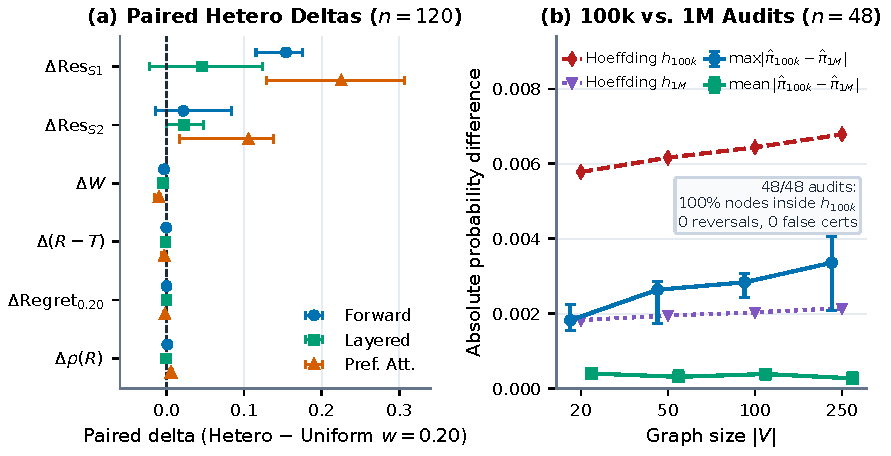
\includegraphics[width=0.96\textwidth]{figures/v2/fig_v2_hetero_and_precision_audit.pdf}
\caption{Weight-heterogeneity sensitivity ($120$ paired heterogeneous vs.\ uniform $w=0.20$ evaluations) and independent $N=1{,}000{,}000$-trial Monte Carlo precision audits ($48$ low-weight scenarios).}
\label{fig:v2-hetero-audits}
\end{figure}

Table~\ref{tab:v2-hetero-audits} (Part~A) and
Figure~\ref{fig:v2-hetero-audits} show that introducing edge-weight
heterogeneity around the same mean weight $0.20$ \textbf{improved}
rather than degraded GBBRPM's bracket tightness, ranking accuracy, and
screening resolution across all three topology families. Across the
$60$ paired graph replicates ($120$ scenario pairs), heterogeneous
weights reduced mean scalar width by $\Delta W = -0.00702$ ($-0.0070$,
largest in Preferential Attachment at $-0.0125$), reduced tree width by
$\Delta(R-T) = -0.0025$, kept upper slack virtually unchanged
($\Delta(R-\pi) = -0.00005$), lowered $f=0.20$ selection regret by
$\Delta\mathrm{Regret}_{R,0.20} = -0.00112$ (and reduced $M_j$ regret
by $-0.4260$), increased Spearman $\rho(R)$ by $+0.0023$, and boosted
Stage~1 screening resolution by $+14.9\text{ pp}$ and Stage~2 resolution
by $+3.27\text{ pp}$ ($+3.3\text{ pp}$), with zero reversals in both
matched conditions. Weight heterogeneity breaks near-ties among
candidate paths, confirming that the primary uniform-weight grid acts as
a conservative stress test rather than an artificially favorable regime.

Table~\ref{tab:v2-hetero-audits} (Part~B) confirms that $N=100{,}000$
Monte Carlo sampling noise did not distort any held-out conclusion.
Increasing trials tenfold to $N=1{,}000{,}000$ contracted the union-bound
Hoeffding half-width by $\sqrt{10}\times$ from mean $h_{100k}=0.0063$
($0.0058$--$0.0068$) to $h_{1M}=0.0020$ ($0.0018$--$0.0021$). Across
all $48$ independent audits, \textbf{$100.0\%$} of $1\text{M}$ node
estimates lay inside the $100\text{k}$ Hoeffding CI (and $100.0\%$
within the combined $h_{100k}+h_{1M}$ interval), $97.34\%$ ($97.3\%$) of
$100\text{k}$ estimates lay inside the tighter $1\text{M}$ CI, maximum
single-node discrepancy across all audited nodes was $0.00475$
($0.004752$; mean of scenario maxima $0.00257$), and mean absolute
discrepancy was $0.000375$ ($0.00038$). Tighter $1\text{M}$ intervals
resolved $+2,213$ additional strict model pairs ($305,552 \to 307,765$;
resolved fraction $91.70\% \to 92.37\%$) while recording \textbf{zero}
reversals, \textbf{zero} false certifications, and \textbf{zero} empty
Hoeffding intersections at both precisions.

\subsection{Computational Scalability and Memory Tradeoffs}
\label{sec:v2-scalability}

Hypothesis~$H_5$ was evaluated through an isolated $158$-row
computational benchmark ($5$ warm-up passes, $30$ measured
\texttt{time.perf\_counter()} repetitions, and separate post-GC
\texttt{tracemalloc} peak Python heap passes so profiling overhead
never perturbed wall-clock timings). The benchmark spanned a sparse DAG
series ($|V| \in \{20, 50, 100, 250, 500, 1000\}$, $|E| = 3|V|$), a
dense DAG stress series ($|V| \in \{20, 50, 100, 250\}$, $25\%$ edge
density up to $|E| = 7,781$), and a paired $100\text{k}$ bit-packed
Monte Carlo reference series on held-out Forward DAGs
(seed~\texttt{1001}, $w=0.50$, $B=0.50$, $5$ MC repetitions).

% Auto-generated by scripts/generate_paper_outputs.py --target thesis; do not edit manually.
\begin{table}[htbp]
\centering
\caption{Computational runtime (median [IQR] ms) and peak Python heap memory across sparse, dense, and paired 100k MC benchmarks.}
\label{tab:v2-scalability}
\footnotesize
\setlength{\tabcolsep}{4.0pt}
\resizebox{\linewidth}{!}{%
\begin{tabular}{lrrrrrrr}
\toprule
$|V| / |E|$ & CSR & Core DF & Abbe / MC & Anc. / CSR$\times$ & 2-Stage / 2S$\times$ & Full $T_j$ / Thr. & Peak Mem. \\
\midrule
\multicolumn{8}{l}{\textbf{Sparse Series ($|E|=3|V|$, seed=41; 30 reps): Median [IQR] ms}} \\
\midrule
20 / 60 & 0.058 [0.014] & 13.23 [6.00] & 0.151 [0.010] & 0.212 [0.069] & 1.27 [0.28] & 0.903 [0.226] & 0.5 KB \\
50 / 150 & 0.147 [0.006] & 16.74 [7.75] & 0.611 [1.696] & 0.468 [0.301] & 4.33 [0.86] & 4.67 [2.72] & 0.7 KB \\
100 / 300 & 0.286 [0.040] & 18.61 [19.43] & 0.638 [0.078] & 0.922 [0.395] & 15.33 [1.97] & 14.48 [2.86] & 1.2 KB \\
250 / 750 & 0.737 [0.099] & 29.91 [8.13] & 1.88 [0.74] & 2.40 [0.32] & 112.4 [51.4] & 88.14 [27.19] & 2.4 KB \\
500 / 1500 & 1.81 [1.58] & 61.00 [31.53] & 4.22 [0.62] & 6.96 [1.99] & 279.1 [35.7] & 343.4 [54.5] & 4.4 KB \\
1000 / 3000 & 3.27 [0.61] & 131.2 [35.9] & 9.45 [3.07] & 13.30 [2.48] & 458.1 [54.8] & 1225.0 [963.3] & 8.3 KB \\
\midrule
\multicolumn{8}{l}{\textbf{Dense Series (25\% DAG density, seed=41; 30 reps): Median [IQR] ms}} \\
\midrule
20 / 47 & 0.020 [0.000] & 4.12 [0.68] & 0.051 [0.009] & 0.095 [0.007] & 0.509 [0.145] & 0.452 [0.114] & 0.5 KB \\
50 / 306 & 0.096 [0.013] & 5.85 [0.76] & 0.459 [0.159] & 0.489 [0.090] & 3.90 [1.25] & 3.11 [0.67] & 0.8 KB \\
100 / 1237 & 0.475 [0.323] & 11.91 [2.34] & 1.39 [0.54] & 5.06 [0.61] & 24.23 [3.22] & 23.63 [5.44] & 1.2 KB \\
250 / 7781 & 2.52 [0.60] & 55.66 [3.30] & 5.62 [0.53] & 63.91 [5.57] & 290.6 [20.4] & 290.3 [36.5] & 2.4 KB \\
\midrule
\multicolumn{8}{l}{\textbf{Paired 100k MC Reference (Forward, seed=1001, $w=0.50, B=0.50$; 5 MC reps)}} \\
\midrule
20 / 40 & 0.019 ms & 3.67 ms & MC: 16.4 ms & CSR: 879$\times$ & 2-Stg: 19.6$\times$ & 245M e-tr/s & 3.7 MB (MC) \\
50 / 100 & 0.046 ms & 4.25 ms & MC: 44.2 ms & CSR: 959$\times$ & 2-Stg: 28.0$\times$ & 226M e-tr/s & 9.1 MB (MC) \\
100 / 200 & 0.090 ms & 4.27 ms & MC: 99.7 ms & CSR: 1103$\times$ & 2-Stg: 24.3$\times$ & 201M e-tr/s & 18.3 MB (MC) \\
250 / 500 & 0.246 ms & 6.25 ms & MC: 268.8 ms & CSR: 1094$\times$ & 2-Stg: 17.1$\times$ & 186M e-tr/s & 45.7 MB (MC) \\
\bottomrule
\end{tabular}
}
\par\vspace{3pt}\parbox{0.98\linewidth}{\raggedright\scriptsize Log-log scaling vs. $|V|+|E|$: GBBRPM (CSR) achieves near-linear exponent $b=1.045$ ($R^2=0.9982$) on sparse and $b=1.022$ ($R^2=0.9974$) on dense DAGs, whereas full-graph $T_j$ scales at $b=1.853$ ($R^2=0.9992$). Peak memory measured via isolated \texttt{tracemalloc} passes.}
\end{table}


\begin{figure}[htbp]
\centering
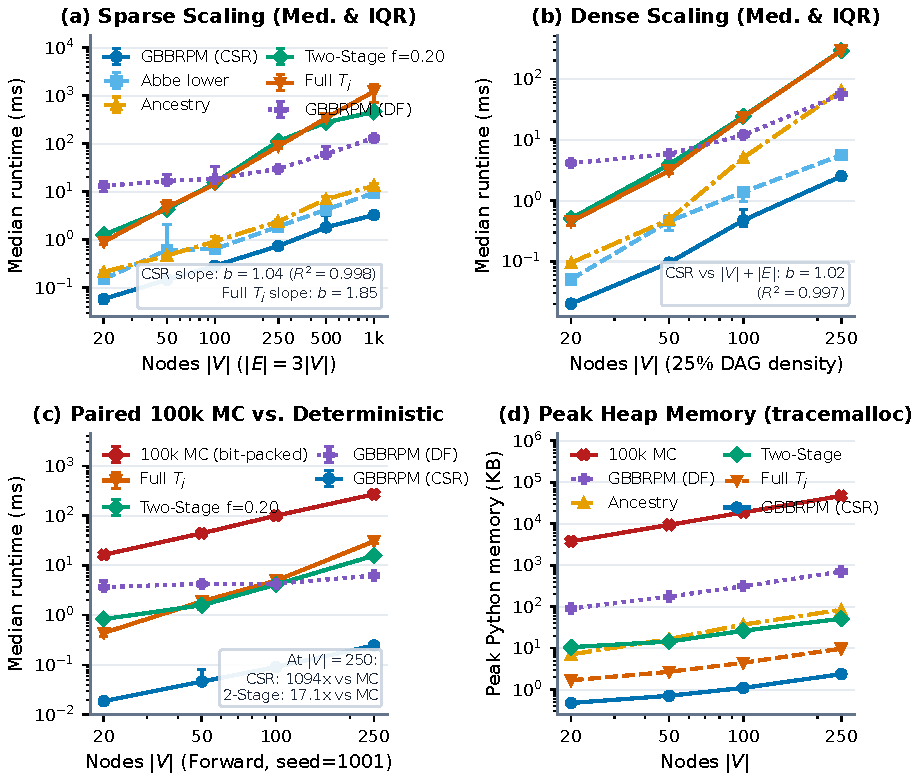
\includegraphics[width=0.96\textwidth]{figures/v2/fig_v2_scalability_sparse_dense.pdf}
\caption{Empirical runtime scaling (median ms with log-log power-law fits against $|V|+|E|$) and isolated peak Python heap memory across sparse DAGs ($|V|=20\dots 1000$), dense DAGs ($25\%$ density), and paired $N=100{,}000$ bit-packed Monte Carlo references.}
\label{fig:v2-scalability}
\end{figure}

Table~\ref{tab:v2-scalability} and Figure~\ref{fig:v2-scalability}
confirm near-linear complexity for the CSR propagation core alongside
clear cost boundaries for heavier comparators:
\begin{itemize}[leftmargin=*]
\item \textbf{Near-Linear CSR Propagation and Low Heap Footprint.} On
sparse DAGs ($|V| = 20 \dots 1000$), single-pass CSR GBBRPM runtime
scaled from $0.058\text{ ms}$ (IQR $0.014\text{ ms}$) to
$3.27\text{ ms}$ (IQR $0.61\text{ ms}$) with empirical log-log power-law
exponent $b = 1.045$ ($R^2 = 0.9982$) against $|V|+|E|$ and peak Python
heap memory of only $8.3\text{ KB}$ at $|V|=1000$ ($0.5\text{ KB}$ at
$|V|=20$). On dense DAGs up to $|V|=250, |E|=7,781$, CSR propagation
remained near-linear at $b = 1.022$ ($R^2 = 0.9974$, median
$2.52\text{ ms}$, peak heap $2.4\text{ KB}$). Complete ranking added
only $0.752\text{ ms}$ ($37.7\text{ KB}$) at $|V|=1000$.
\item \textbf{Wrapper Overhead vs.\ Algorithmic Complexity.} The
traceable pandas DataFrame API (\texttt{gbbrpm\_core\_df}), which
constructs full edge-contribution tables and schema metadata for the
prototype, required $13.23\text{ ms}$ ($114.6\text{ KB}$) at $|V|=20$
and $131.2\text{ ms}$ ($3,799\text{ KB}$) at $|V|=1000$ (with graph
validation/preparation taking $7.06$--$27.69\text{ ms}$). Separating
one-time validation from CSR propagation is therefore essential for
batch sweeps and screening.
\item \textbf{Super-Linear Growth of Full $T_j$ and Dense Ancestry vs.\
Two-Stage Screening.} Computing full-graph target-specific trees $T_j$
for every node scaled super-linearly on sparse DAGs at $b = 1.853$
($R^2 = 0.9992$), reaching $1,225.0\text{ ms}$ at $|V|=1000$
($375\times$ slower than CSR $R_j$). Two-Stage Certified Screening at
$f=0.20$ cut $|V|=1000$ runtime by $2.67\times$ to $458.1\text{ ms}$
($229.0\text{ KB}$). On dense DAGs ($|V|=250, |E|=7,781$), the
connected-component ancestry diagnostic escalated sharply to
$63.91\text{ ms}$ ($b = 1.390$, $523.8\text{ KB}$), whereas CSR $R_j$
stayed at $2.52\text{ ms}$ and \citet{abbe2020} at $5.62\text{ ms}$.
\item \textbf{Paired $100\text{k}$ Monte Carlo Speedups and Cost
Caveat.} Against vectorized bit-packed $100\text{k}$ Monte Carlo
($16.4\text{ ms}$--$268.8\text{ ms}$, throughput $186$--$245\text{M}$
edge-trials/s, peak heap $3.7$--$45.7\text{ MB}$), CSR GBBRPM achieved
\textbf{$879\times$--$1,103\times$} wall-clock speedups ($879\times$ at
$|V|=20$, $959\times$ at $|V|=50$, $1,103\times$ at $|V|=100$,
$1,094\times$ at $|V|=250$) with $>1{,}500\times$ lower peak heap
allocation, while Two-Stage Certified Screening achieved
\textbf{$17.1\times$--$28.0\times$} speedups with deterministic
soundness. Consistent with Chapter~1, these speedups reflect a static,
local-state scalar DAG pass and do not establish computational
equivalence to hydrodynamic or AC power-flow simulators.
\end{itemize}

\subsection{Eligible Real-Domain Instantiations and Evidence Boundaries}
\label{sec:v2-domain-cases}

Three real-data instantiations were evaluated independently using the
identical frozen GBBRPM core while preserving strict non-pooling across
domains, explicit Gate~A (structural readiness) and Gate~B (independent
outcome validation) status, and strict privacy/redistribution boundaries.
Zero bracket violations, zero Abbe violations, and zero false
certifications occurred across all $115$ real-domain scenario runs
(plus the $12$ stochastic \texttt{Express 4.18.2} benchmark runs).

% Auto-generated by scripts/generate_paper_outputs.py --target thesis; do not edit manually.
\begin{table}[htbp]
\centering
\caption{Strictly non-pooled cross-domain mechanism synthesis, eligibility gates, and evidence boundaries.}
\label{tab:v2-domain-cases}
\footnotesize
\setlength{\tabcolsep}{4.0pt}
\resizebox{\linewidth}{!}{%
\begin{tabular}{llccc p{4.6cm} p{3.6cm}}
\toprule
Domain & Case & $|V|/|E|$ & Gate A / B & Scen. & Key verified mechanism finding & Evidence boundary \\
\midrule
Urban Drainage & DPWH CDO Bitan-ag--Kolambog & 11 / 11 (Reconv.) & PASS / FAIL & 67 & $S \in [0.464, 0.847]$; J\_AGORA\_CONF max $R-\pi=0.0511$; S2 res. 98.8\% & Restricted agency data; Tier-2 exploratory only (no field-flood validation) \\
Software Dependency & npm Express 4.18.2 (OSV) & 71 / 128 (Reconv.) & PASS / N/A & 5 ($\tau$) + 12 (stoch.) & Root $R(\tau=1)=0.997528$ (exact $\pi=0.993408$); isolated qs $R-\pi=0.250$, send $0.188$ & Public lockfile/OSV; advisories define inputs $B_i$, not exploit outcomes \\
Electrical Distribution & Caltech SoCal 28-Bus Comp. 2 & 12 / 11 (Tree) & PASS / FAIL & 43 & Verified arborescence: 43/43 exact with $\max|R-\pi|=2.2\times 10^{-16} < 10^{-12}$, $\max|T-R|=0.0$ & Restricted telemetry (post-event normal window); no fault-prediction claim \\
\bottomrule
\end{tabular}
}
\par\vspace{3pt}\parbox{0.98\linewidth}{\raggedright\scriptsize All three domains exhibit 0 bracket violations, 0 Abbe violations, and 0 false certifications. No raw DPWH conduit tables, no raw Caltech phasor measurements, and no PII are exported; metrics are strictly non-pooled across domains.}
\end{table}


\begin{figure}[htbp]
\centering
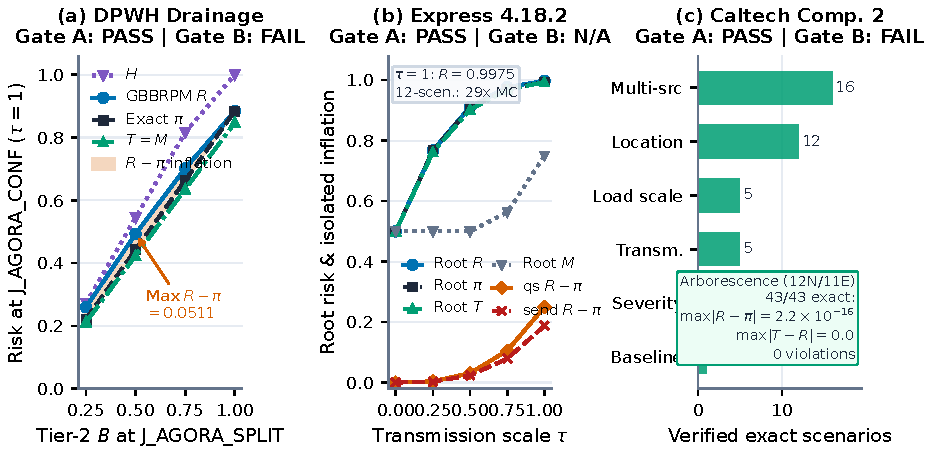
\includegraphics[width=0.96\textwidth]{figures/v2/fig_v2_domain_synthesis.pdf}
\caption{Strictly non-pooled cross-domain mechanism synthesis across the three Gate~A eligible topologies: (a)~DPWH Cagayan de Oro Bitan-ag--Kolambog drainage reach reconvergence at \texttt{J\_AGORA\_CONF} (Gate~B FAIL), (b)~\texttt{npm:express@4.18.2} transmission sweep and isolated \texttt{qs}/\texttt{send} reconvergence (Gate~B N/A), and (c)~\texttt{Caltech SoCal 28-Bus} Component~2 exact arborescence verification (Gate~B FAIL).}
\label{fig:v2-domain-synthesis}
\end{figure}

Table~\ref{tab:v2-domain-cases} and Figure~\ref{fig:v2-domain-synthesis}
summarize the verified mechanism findings and non-negotiable evidence
boundaries of each domain.

\subsubsection{Urban Drainage: DPWH Cagayan de Oro Bitan-ag--Kolambog Reach (Gate~A PASS / Gate~B FAIL)}

Constructed from the official DPWH Regional Office~X FOI release
(\texttt{FOI-REQ-2026-7383}; \citealp{dpwh2026foi,upplanades2016}), the
verified Bitan-ag--Kolambog DAG
(\texttt{drainage\_\allowbreak dpwh\_\allowbreak cdo\_\allowbreak bitanag\_\allowbreak kolambog\_\allowbreak v1})
comprises $11$ junctions and $11$ directed drainage conduits with
heterogeneous engineering load-to-capacity susceptibilities
$S_{ij} \in [0.4639, 0.8471]$ (mean $0.6417$, Manning conveyance checks
within $1\%$) and a real physical reconvergence diamond where the Agora
diversion split (\texttt{J\_AGORA\_SPLIT}) bifurcates into the two-hop
main Bitan-ag trunk (via \texttt{J\_TRIB1\_CONF}) and the one-hop Agora
diversion channel before reconverging at \texttt{J\_AGORA\_CONF}
(PCSWMM junction \texttt{J5}).

Across $67$ Tier-2 controlled blockage scenarios ($63$ solved by exact
enumeration and $4$ all-node stress runs by $100\text{k}$ MC fallback;
zero violations and zero DataFrame-vs.-CSR parity error), GBBRPM
captured real heterogeneous $L/C$ propagation and quantified exact
shared-ancestry inflation at \texttt{J\_AGORA\_CONF}. Positive upper
slack ($R_j > \pi_j$) occurred in $49/63$ exact scenarios, peaking at
$R - \pi = 0.05108$ ($0.051080$, with $R = 0.4931$, exact $\pi = 0.4420$,
$T = M = 0.4236$, $W = 0.0695$) under single-source injection at
\texttt{J\_AGORA\_SPLIT} ($B = 0.50, \tau = 1.00$), and collapsing
identically to $R - \pi = 0.0$ when the split disturbance became
deterministic ($B = 1.00$, $R = \pi = 0.8840$). Under headwater
injection (\texttt{J\_BIT\_HEAD}, $\tau=1.00$), upper slack rose
smoothly from $0.0187$ ($B=0.25$) to $0.0493$ ($B=1.00$, because
upstream attenuation makes the split arrival uncertain even at $B=1.00$),
while the ancestry diagnostic differed from $R$ by up to $0.2105$ in
all-headwaters scenarios. Two-Stage Certified Screening at $f=0.20$
resolved $94.3\%$ of candidates in Stage~1 and $98.8\%$ ($0.9881$) in
Stage~2.

\textbf{Evidence Boundary (Gate~B FAIL).} Consistent with
Table~\ref{tab:domain-contingency}, these $67$ runs verify only
structural DAG instantiation, heterogeneous $L/C$ propagation, and
real-topology reconvergence mechanics. Because the June~10, 2025 CDO
2nd~DEO flood-hotspot inspection records (\texttt{B01--B16}) reflect
existing-channel conditions rather than the 2016 Master Plan diversion
geometry and lack non-flooded controls and pre-event blockage
measurements, \textbf{no confirmatory field-flooding validation claim
is made}. Furthermore, historical exploratory SWMM comparisons
(\hyperref[app:preliminary]{Appendix D}) demonstrated that backwater,
surcharge, and upstream ponding fall outside a strictly downstream
static DAG model. No raw DPWH conduit tables or personally identifiable
information were exported to the repository or manuscript.

\subsubsection{Software Dependency: \texttt{npm:express@4.18.2} (Gate~A PASS / Gate~B N/A)}

The verified public software dependency DAG
(\texttt{software\_\allowbreak npm\_\allowbreak express\_\allowbreak 4.18.2}; $71$ exact package-version
nodes, $128$ reversed dependency edges, $7$ OSV advisory roots,
SHA-256 verified against the frozen manifest) confirmed coherent
real-topology instantiation across a $5$-point deterministic
transmission sweep ($\tau \in \{0.00, 0.25, 0.50, 0.75, 1.00\}$) and
the $12$-scenario held-out stochastic suite. At $\tau = 1.00$, GBBRPM
reproduced the exact verified root risk
$R(\texttt{npm:express@4.18.2}) = 0.997528076171875$ against exact
enumeration $\pi = 0.993408203125$ (combined upper slack
$R - \pi = 0.004120$, scalar width $W = 0.2475$), with the root
ascending from rank~$3$ at $\tau = 0.00$ ($R = 0.5000$) to rank~$1$ by
$\tau = 0.50$ ($R = 0.9118$).

Isolating individual reconvergent dependency diamonds revealed
substantial latent overlap masked by multi-root saturation in the
combined graph: \texttt{npm:qs@6.11.0} reaches \texttt{express@4.18.2}
both directly and via \texttt{body-parser@1.20.1}, producing an
isolated exact upper slack of $R - \pi = 0.2500$ ($R = 0.7500$ vs.\
$\pi = 0.5000$) at $\tau = 1.00$, while \texttt{npm:send@0.18.0}
reaches the root directly and via \texttt{serve-static@1.15.0},
producing an isolated exact upper slack of $R - \pi = 0.1875$
($R = 0.4375$ vs.\ $\pi = 0.2500$).

An important structural transparency note emerged from the $12$-scenario
held-out stochastic benchmark (\texttt{heldout\_express\_12}, uniform
$w \in \{0.05, 0.10, 0.20, 0.25, 0.50, 0.75\}$, $B \in \{0.50, 1.00\}$):
because all $7$ OSV advisory roots (\texttt{cookie},
\texttt{path-to-regexp}, \texttt{qs}, \texttt{send} $\to$
\texttt{body-parser}, \texttt{serve-static} $\to$ \texttt{express@4.18.2})
occupy the top-most dependent subgraph of the reversed dependency DAG,
\textbf{$0/64$ non-advisory packages} ($C = \{B_j = 0\}$) lie
downstream of any advisory root. Consequently, strict candidate-set
($C$) metrics are identically zero ($W=0, R=\pi=0$), whereas
non-trivial stochastic reconvergence occurs within the $7$-node
advisory subgraph and root package: at $B=0.50$, root scalar width
$W(\texttt{express})$ spanned $0.0710$ ($w=0.05$) to $0.4821$
($w=0.75$) with mean tree width $0.00707$ and maximum upper slack
$0.00630$ ($0.0063$).

\textbf{Evidence Boundary (Gate~B N/A).} OSV advisory severities define
the local disturbance inputs $B_i$, not independent exploitation or
incident outcome labels. The software case establishes structural
instantiation and quantifies reconvergence sensitivity; it makes
\textbf{no claim of software exploit prediction}.

\subsubsection{Electrical Distribution: Caltech SoCal 28-Bus Component~2 (Gate~A PASS / Gate~B FAIL)}

The verified Component~2 radial feeder from the Caltech SoCal 28-Bus
dataset \citep{xie2025} (\texttt{electrical\_\allowbreak caltech\_\allowbreak socal28\_\allowbreak component2}:
$12$ nodes, $11$ directed edges, $24$ phasor snapshots, baseline
measured load-to-capacity susceptibilities $S_{ij} \in [0.0139, 0.3949]$,
mean $0.1909$) is a strict directed arborescence ($\max$ in-degree $= 1$,
zero reconvergent nodes). Across all $43$ exact scenarios spanning
single-node disturbances, root severities, load scales, transmission
levels, and multi-source pairs, the evaluation confirmed theoretical
tree equivalence to machine precision: $\max |R_j - \pi_j| =
2.22 \times 10^{-16} < 10^{-12}$, $\max |T_j - R_j| = 0.0$,
$\max |R_j - \text{Ancestry}_j| = 0.0$, and zero bracket or
certification violations, with aggregate network risk sum ranging from
$0.0$ to $3.7544$ and Two-Stage Screening resolving $75.3\%$ of
candidates identically in Stage~1 and Stage~2.

\textbf{Evidence Boundary (Gate~B FAIL).} Because the authorized
telemetry covers a normal-operation window following the November~13,
2024 switching event without aligned fault or outage labels, this case
verifies radial arborescence instantiation and exact tree equivalence
only; \textbf{no operational fault-prediction or switching-response
claim is made}, and raw phasor measurements remain strictly outside
version control.

\subsection{Synthesis Against Research Hypotheses (\texorpdfstring{$H_1$--$H_5$}{H1--H5}) and Threats to Validity}
\label{sec:v2-synthesis-threats}

Table~\ref{tab:v2-hypothesis-verdict} maps the confirmatory v2.0.0
empirical findings directly onto the five falsifiable research
hypotheses ($H_1$--$H_5$) stated in Section~\ref{research-hypotheses}
and the evaluation criteria of Table~\ref{tab:evaluation-criteria}.

\begin{table}[htbp]
\centering
\caption{Confirmatory empirical verdicts against Research Hypotheses $H_1$--$H_5$ (frozen \texttt{v2.0.0-heldout-eval} evidence).}
\label{tab:v2-hypothesis-verdict}
\footnotesize
\renewcommand{\arraystretch}{1.14}
\begin{tabularx}{\textwidth}{@{}>{\raggedright\arraybackslash}p{2.35cm} >{\raggedright\arraybackslash}p{2.05cm} L@{}}
\toprule
Hypothesis & Verdict & Confirmatory Evidence and Boundary Conditions \\
\midrule
\textbf{$H_1$: Bracket Tightness \& Dependence} &
\textbf{Supported} &
Matched controls ($n=560$): exact equivalence on independent origins ($\max|R-\pi|=1.11\times 10^{-16}$), shared-origin upper slack up to $0.6499$ at $0<b<1$, exact collapse to $0.0$ at $b=1$. Held-out DAGs ($n=2,880$): mean $R-\pi = 0.0060$ ($86.7\%$ of $R-T=0.0450$ is lower slack $\pi-T=0.0390$); $R-\pi$ scales monotonically with $w$ ($<2\times 10^{-5}$ at $w\le 0.10$ to $0.0222$ at $w=0.75$) and is $9.1\times$ larger at $B=0.50$ than $B=1.00$. \\
\addlinespace
\textbf{$H_2$: Fixed-Budget Selection vs.\ Comparators} &
\textbf{Supported} (with high-overlap reversal caveat) &
At $f=0.20$ ($n=240$ replicates), $R_j$ achieved lowest regret ($0.00742$), highest capture ($50.59\%$), and highest Spearman $\rho$ ($0.9833$), strictly beating $T_j$ ($0.1483$, $97.5\%$ wins), $H_j$ ($0.2889$, $100.0\%$ wins; avoids $H_j$'s $16.29\%$ $\ge 0.95$ saturation), Abbe ($0.2968$, $98.3\%$), ancestry ($0.5590$, $99.6\%$), local-upstream ($0.9185$, $98.8\%$), and $M_j$ ($0.9332$, $99.6\%$). Honest caveat: interval-resolved reversals occurred in $696/2,880$ scenarios (pooled rate $0.198\%$), concentrated at $w \in \{0.50, 0.75\}$ and $B=0.50$, with $13.30\%$ unresolved pairs at $100\text{k}$ MC. \\
\addlinespace
\textbf{$H_3$: Two-Stage Certified Screening} &
\textbf{Supported} &
Zero false certifications across $8,640$ held-out evaluations. At $f=0.20$, deterministic resolution jumped from $\mathrm{Res}_{S1}=47.5\%$ to $\mathrm{Res}_{S2}=78.9\%$ ($+31.5\text{ pp}$ contraction) and full certification from $2.43\%$ to $16.25\%$, delivering $2.00\times$ aggregate speedup over full $T_j$ (replicate median $2.24\times$) and $18.6\times$ over $100\text{k}$ MC (scenario median $43.3\times$). Resolution drops to $53.75\%$ at $w=0.75$, delineating where MC escalation remains necessary. \\
\addlinespace
\textbf{$H_4$: $W_j$ Width Self-Diagnosis} &
\textbf{Partially Supported} &
Strong as a scenario-level reversal alarm: Spearman($W_{\max}$, reversal rate) $= 0.6769$ with $100.0\%$ recall ($0$ false negatives) at $W_{\max}\ge 0.10$ ($72.6\%$ flagged). Weak for within-graph nodewise slack ranking ($\rho = 0.2286$) and continuous regret ($\rho = 0.2815$), because $W_j$ mixes small upper slack ($0.0060$) with $18\times$ larger legitimate multi-branch convergence ($\pi-M=0.1065$). \\
\addlinespace
\textbf{$H_5$: Near-Linear Scaling \& Cost} &
\textbf{Supported} &
CSR propagation scaled near-linearly against $|V|+|E|$ on sparse DAGs ($|V|=20\dots 1000$: $0.058\to 3.27\text{ ms}$, $b=1.045$, $R^2=0.9982$, $8.3\text{ KB}$) and dense DAGs ($|V|\le 250, |E|\le 7,781$: $b=1.022$, $R^2=0.9974$, $2.4\text{ KB}$), versus full $T_j$ ($b=1.853$, $1,225\text{ ms}$). Paired $100\text{k}$ MC speedups reached $879\times$--$1,103\times$ (CSR) and $17.1\times$--$28.0\times$ (Two-Stage Screening). \\
\bottomrule
\end{tabularx}
\end{table}

\subsubsection{Threats to Validity}

Five classes of threats constrain the interpretation of these results:
\begin{enumerate}[label=\arabic*.,leftmargin=*]
\item \textbf{Construct Validity (Stochastic Reference vs.\ Domain
Semantics).} The controlled benchmark defines exact probabilities $\pi_j$
under independent Bernoulli source and edge primitives (Equation~3-10).
Real drainage blockage ratios, OSV advisory severities, and electrical
loading ratios are bounded domain indices rather than calibrated
independent probabilities; tight agreement with $\pi_j$ validates the
propagation mechanism under its declared reference, not physical
probability calibration.
\item \textbf{Internal Validity (Finite-Sample MC Resolution and
Unresolved Pairs).} Although the $48$ independent $1\text{M}$-trial
audits confirmed $100.0\%$ inclusion inside $100\text{k}$ Hoeffding
intervals ($\max|\Delta\hat{\pi}|=0.00475$, zero reversals), $13.30\%$
of candidate pairs in the primary $2,880$-scenario suite lay within the
$N=100{,}000$ Hoeffding margin ($h \approx 0.0063$). All interval-based
claims treat those pairs explicitly as unresolved rather than asserting
strict order.
\item \textbf{External Validity (DAG Scope and Domain Gate~B Limits).}
The frozen core rejects directed cycles, bidirectional backwater, and
meshed loops by fail-closed design. None of the three real-domain
topologies passed Gate~B independent outcome validation (DPWH and
Caltech failed Gate~B; Express was Gate~B N/A), so real-world
operational prioritization utility remains unestablished pending
field-verified outcome datasets.
\item \textbf{Statistical Conclusion Validity (Single-Topology Timing
and Replicate Dependence).} Held-out benchmark means and standard
deviations were aggregated over independent graph replicates ($n=240$
uniform; $n=60$ heterogeneous) to prevent pseudo-replication across
correlated $(w, B)$ sweeps. Scalability fits were measured on one
Windows~11 AMD64 workstation; absolute millisecond constants will vary
across hardware, though asymptotic slopes ($b \approx 1.02$--$1.05$ for
CSR vs.\ $1.85$ for full $T_j$) reflect structural complexity.
\item \textbf{Prototype Scope Validity.} Automated functional
verification ($76/76$ prototype tests) established numerical parity,
fail-closed validation, and replay traceability in the tested
environment, not end-user usability, multi-user concurrency, or
production security hardening.
\end{enumerate}
